\documentclass{standalone}
\usepackage{tikz}
\usepackage{xcolor}
\usetikzlibrary{patterns, positioning}

    \usetikzlibrary{calc}
    \usepackage{relsize}
    \tikzset{fontscale/.style = {font=\relsize{#1}}}
\begin{document}
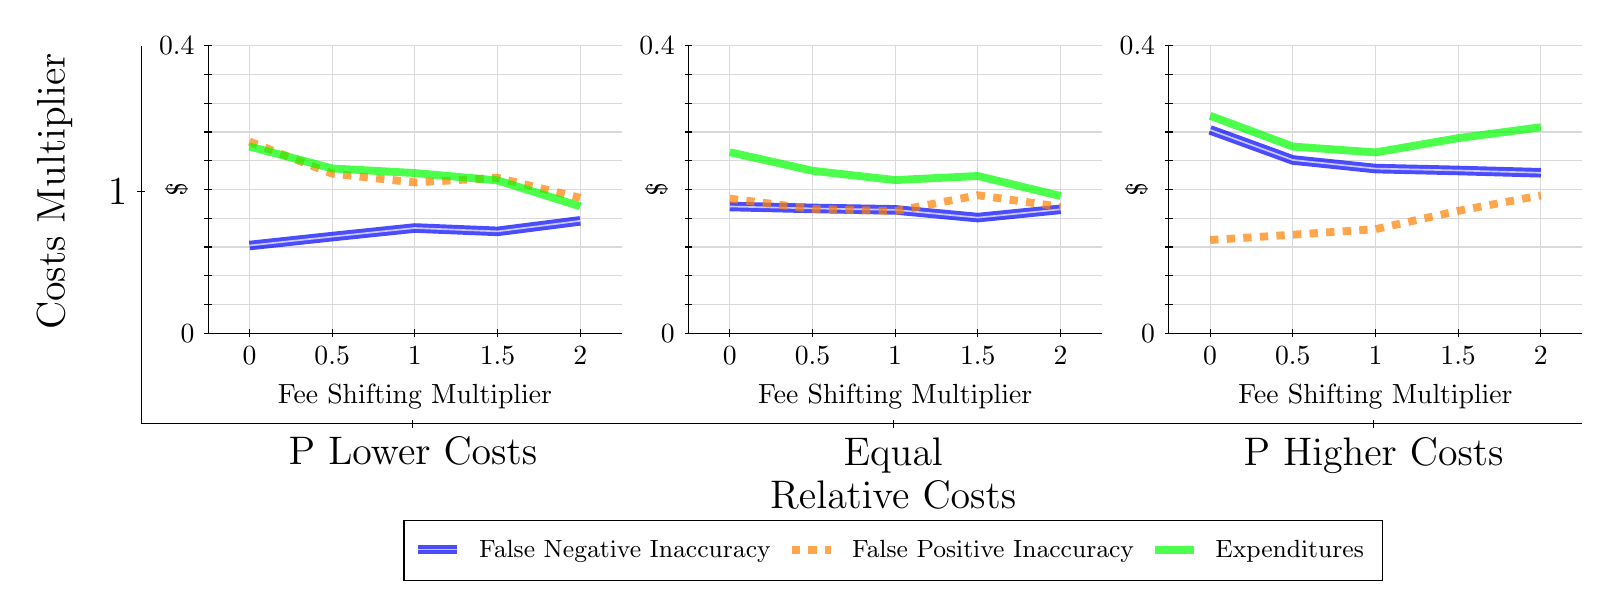
\begin{tikzpicture}
\draw[black] (1.7,1.5) -- (1.7,6.3);
\node[rotate=90, fontscale=2, anchor=center] at (0.6, 4.45) {Costs Multiplier};
\draw[black] (1.65,4.45) -- (1.75,4.45);
\node[fontscale=2, anchor=east] at (1.65, 4.45) {1};

\draw[black] (1.7,1.5) -- (20,1.5);
\node[fontscale=2, anchor=center] at (11.25, 0.6) {Relative Costs};
\draw[black] (5.15,1.45) -- (5.15,1.55);
\node[fontscale=2, anchor=north] at (5.15, 1.45) {P Lower Costs};
\draw[black] (11.25,1.45) -- (11.25,1.55);
\node[fontscale=2, anchor=north] at (11.25, 1.45) {Equal};
\draw[black] (17.35,1.45) -- (17.35,1.55);
\node[fontscale=2, anchor=north] at (17.35, 1.45) {P Higher Costs};


\draw[gray!30] (2.55,2.65) -- (7.8,2.65);
\draw[gray!30] (2.55,3.015) -- (7.8,3.015);
\draw[gray!30] (2.55,3.38) -- (7.8,3.38);
\draw[gray!30] (2.55,3.745) -- (7.8,3.745);
\draw[gray!30] (2.55,4.11) -- (7.8,4.11);
\draw[gray!30] (2.55,4.475) -- (7.8,4.475);
\draw[gray!30] (2.55,4.84) -- (7.8,4.84);
\draw[gray!30] (2.55,5.205) -- (7.8,5.205);
\draw[gray!30] (2.55,5.57) -- (7.8,5.57);
\draw[gray!30] (2.55,5.935) -- (7.8,5.935);
\draw[gray!30] (2.55,6.3) -- (7.8,6.3);
\draw[gray!30] (3.075,2.65) -- (3.075,6.3);
\draw[gray!30] (4.125,2.65) -- (4.125,6.3);
\draw[gray!30] (5.175,2.65) -- (5.175,6.3);
\draw[gray!30] (6.225,2.65) -- (6.225,6.3);
\draw[gray!30] (7.275,2.65) -- (7.275,6.3);
\draw[black] (2.55,2.65) -- (2.55,6.3);
\node[rotate=90, fontscale=0.7, anchor=center] at (2.15, 4.475) {\$};
\draw[black] (2.5,2.65) -- (2.6,2.65);
\node[fontscale=0.7, anchor=east] at (2.5, 2.65) {0};
\draw[black] (2.5,3.015) -- (2.6,3.015);
\node[fontscale=0.7, anchor=east] at (2.5, 3.015) { };
\draw[black] (2.5,3.38) -- (2.6,3.38);
\node[fontscale=0.7, anchor=east] at (2.5, 3.38) { };
\draw[black] (2.5,3.745) -- (2.6,3.745);
\node[fontscale=0.7, anchor=east] at (2.5, 3.745) { };
\draw[black] (2.5,4.11) -- (2.6,4.11);
\node[fontscale=0.7, anchor=east] at (2.5, 4.11) { };
\draw[black] (2.5,4.475) -- (2.6,4.475);
\node[fontscale=0.7, anchor=east] at (2.5, 4.475) { };
\draw[black] (2.5,4.84) -- (2.6,4.84);
\node[fontscale=0.7, anchor=east] at (2.5, 4.84) { };
\draw[black] (2.5,5.205) -- (2.6,5.205);
\node[fontscale=0.7, anchor=east] at (2.5, 5.205) { };
\draw[black] (2.5,5.57) -- (2.6,5.57);
\node[fontscale=0.7, anchor=east] at (2.5, 5.57) { };
\draw[black] (2.5,5.935) -- (2.6,5.935);
\node[fontscale=0.7, anchor=east] at (2.5, 5.935) { };
\draw[black] (2.5,6.3) -- (2.6,6.3);
\node[fontscale=0.7, anchor=east] at (2.5, 6.3) {0.4};

\draw[black] (2.55,2.65) -- (7.8,2.65);
\node[fontscale=0.7, anchor=center] at (5.175, 1.85) {Fee Shifting Multiplier};
\draw[black] (3.075,2.6) -- (3.075,2.7);
\node[fontscale=0.7, anchor=north] at (3.075, 2.6) {0};
\draw[black] (4.125,2.6) -- (4.125,2.7);
\node[fontscale=0.7, anchor=north] at (4.125, 2.6) {0.5};
\draw[black] (5.175,2.6) -- (5.175,2.7);
\node[fontscale=0.7, anchor=north] at (5.175, 2.6) {1};
\draw[black] (6.225,2.6) -- (6.225,2.7);
\node[fontscale=0.7, anchor=north] at (6.225, 2.6) {1.5};
\draw[black] (7.275,2.6) -- (7.275,2.7);
\node[fontscale=0.7, anchor=north] at (7.275, 2.6) {2};

\draw[blue, opacity=0.70, line width=0.5mm, double] (3.075,3.7634) -- (4.125,3.8767) -- (5.175,3.9861) -- (6.225,3.9433) -- (7.275,4.0772);
\draw[orange, opacity=0.70, line width=1mm, dashed] (3.075,5.0835) -- (4.125,4.6767) -- (5.175,4.5647) -- (6.225,4.6235) -- (7.275,4.3694);
\draw[green, opacity=0.70, line width=1mm, solid] (3.075,5.0212) -- (4.125,4.7426) -- (5.175,4.6841) -- (6.225,4.5907) -- (7.275,4.2615);

\draw[gray!30] (8.65,2.65) -- (13.9,2.65);
\draw[gray!30] (8.65,3.015) -- (13.9,3.015);
\draw[gray!30] (8.65,3.38) -- (13.9,3.38);
\draw[gray!30] (8.65,3.745) -- (13.9,3.745);
\draw[gray!30] (8.65,4.11) -- (13.9,4.11);
\draw[gray!30] (8.65,4.475) -- (13.9,4.475);
\draw[gray!30] (8.65,4.84) -- (13.9,4.84);
\draw[gray!30] (8.65,5.205) -- (13.9,5.205);
\draw[gray!30] (8.65,5.57) -- (13.9,5.57);
\draw[gray!30] (8.65,5.935) -- (13.9,5.935);
\draw[gray!30] (8.65,6.3) -- (13.9,6.3);
\draw[gray!30] (9.175,2.65) -- (9.175,6.3);
\draw[gray!30] (10.225,2.65) -- (10.225,6.3);
\draw[gray!30] (11.275,2.65) -- (11.275,6.3);
\draw[gray!30] (12.325,2.65) -- (12.325,6.3);
\draw[gray!30] (13.375,2.65) -- (13.375,6.3);
\draw[black] (8.65,2.65) -- (8.65,6.3);
\node[rotate=90, fontscale=0.7, anchor=center] at (8.25, 4.475) {\$};
\draw[black] (8.6,2.65) -- (8.7,2.65);
\node[fontscale=0.7, anchor=east] at (8.6, 2.65) {0};
\draw[black] (8.6,3.015) -- (8.7,3.015);
\node[fontscale=0.7, anchor=east] at (8.6, 3.015) { };
\draw[black] (8.6,3.38) -- (8.7,3.38);
\node[fontscale=0.7, anchor=east] at (8.6, 3.38) { };
\draw[black] (8.6,3.745) -- (8.7,3.745);
\node[fontscale=0.7, anchor=east] at (8.6, 3.745) { };
\draw[black] (8.6,4.11) -- (8.7,4.11);
\node[fontscale=0.7, anchor=east] at (8.6, 4.11) { };
\draw[black] (8.6,4.475) -- (8.7,4.475);
\node[fontscale=0.7, anchor=east] at (8.6, 4.475) { };
\draw[black] (8.6,4.84) -- (8.7,4.84);
\node[fontscale=0.7, anchor=east] at (8.6, 4.84) { };
\draw[black] (8.6,5.205) -- (8.7,5.205);
\node[fontscale=0.7, anchor=east] at (8.6, 5.205) { };
\draw[black] (8.6,5.57) -- (8.7,5.57);
\node[fontscale=0.7, anchor=east] at (8.6, 5.57) { };
\draw[black] (8.6,5.935) -- (8.7,5.935);
\node[fontscale=0.7, anchor=east] at (8.6, 5.935) { };
\draw[black] (8.6,6.3) -- (8.7,6.3);
\node[fontscale=0.7, anchor=east] at (8.6, 6.3) {0.4};

\draw[black] (8.65,2.65) -- (13.9,2.65);
\node[fontscale=0.7, anchor=center] at (11.275, 1.85) {Fee Shifting Multiplier};
\draw[black] (9.175,2.6) -- (9.175,2.7);
\node[fontscale=0.7, anchor=north] at (9.175, 2.6) {0};
\draw[black] (10.225,2.6) -- (10.225,2.7);
\node[fontscale=0.7, anchor=north] at (10.225, 2.6) {0.5};
\draw[black] (11.275,2.6) -- (11.275,2.7);
\node[fontscale=0.7, anchor=north] at (11.275, 2.6) {1};
\draw[black] (12.325,2.6) -- (12.325,2.7);
\node[fontscale=0.7, anchor=north] at (12.325, 2.6) {1.5};
\draw[black] (13.375,2.6) -- (13.375,2.7);
\node[fontscale=0.7, anchor=north] at (13.375, 2.6) {2};

\draw[blue, opacity=0.70, line width=0.5mm, double] (9.175,4.2595) -- (10.225,4.2348) -- (11.275,4.2165) -- (12.325,4.1182) -- (13.375,4.2234);
\draw[orange, opacity=0.70, line width=1mm, dashed] (9.175,4.359) -- (10.225,4.2291) -- (11.275,4.2006) -- (12.325,4.402) -- (13.375,4.2558);
\draw[green, opacity=0.70, line width=1mm, solid] (9.175,4.9487) -- (10.225,4.7131) -- (11.275,4.5946) -- (12.325,4.6466) -- (13.375,4.3923);

\draw[gray!30] (14.75,2.65) -- (20,2.65);
\draw[gray!30] (14.75,3.015) -- (20,3.015);
\draw[gray!30] (14.75,3.38) -- (20,3.38);
\draw[gray!30] (14.75,3.745) -- (20,3.745);
\draw[gray!30] (14.75,4.11) -- (20,4.11);
\draw[gray!30] (14.75,4.475) -- (20,4.475);
\draw[gray!30] (14.75,4.84) -- (20,4.84);
\draw[gray!30] (14.75,5.205) -- (20,5.205);
\draw[gray!30] (14.75,5.57) -- (20,5.57);
\draw[gray!30] (14.75,5.935) -- (20,5.935);
\draw[gray!30] (14.75,6.3) -- (20,6.3);
\draw[gray!30] (15.275,2.65) -- (15.275,6.3);
\draw[gray!30] (16.325,2.65) -- (16.325,6.3);
\draw[gray!30] (17.375,2.65) -- (17.375,6.3);
\draw[gray!30] (18.425,2.65) -- (18.425,6.3);
\draw[gray!30] (19.475,2.65) -- (19.475,6.3);
\draw[black] (14.75,2.65) -- (14.75,6.3);
\node[rotate=90, fontscale=0.7, anchor=center] at (14.35, 4.475) {\$};
\draw[black] (14.7,2.65) -- (14.8,2.65);
\node[fontscale=0.7, anchor=east] at (14.7, 2.65) {0};
\draw[black] (14.7,3.015) -- (14.8,3.015);
\node[fontscale=0.7, anchor=east] at (14.7, 3.015) { };
\draw[black] (14.7,3.38) -- (14.8,3.38);
\node[fontscale=0.7, anchor=east] at (14.7, 3.38) { };
\draw[black] (14.7,3.745) -- (14.8,3.745);
\node[fontscale=0.7, anchor=east] at (14.7, 3.745) { };
\draw[black] (14.7,4.11) -- (14.8,4.11);
\node[fontscale=0.7, anchor=east] at (14.7, 4.11) { };
\draw[black] (14.7,4.475) -- (14.8,4.475);
\node[fontscale=0.7, anchor=east] at (14.7, 4.475) { };
\draw[black] (14.7,4.84) -- (14.8,4.84);
\node[fontscale=0.7, anchor=east] at (14.7, 4.84) { };
\draw[black] (14.7,5.205) -- (14.8,5.205);
\node[fontscale=0.7, anchor=east] at (14.7, 5.205) { };
\draw[black] (14.7,5.57) -- (14.8,5.57);
\node[fontscale=0.7, anchor=east] at (14.7, 5.57) { };
\draw[black] (14.7,5.935) -- (14.8,5.935);
\node[fontscale=0.7, anchor=east] at (14.7, 5.935) { };
\draw[black] (14.7,6.3) -- (14.8,6.3);
\node[fontscale=0.7, anchor=east] at (14.7, 6.3) {0.4};

\draw[black] (14.75,2.65) -- (20,2.65);
\node[fontscale=0.7, anchor=center] at (17.375, 1.85) {Fee Shifting Multiplier};
\draw[black] (15.275,2.6) -- (15.275,2.7);
\node[fontscale=0.7, anchor=north] at (15.275, 2.6) {0};
\draw[black] (16.325,2.6) -- (16.325,2.7);
\node[fontscale=0.7, anchor=north] at (16.325, 2.6) {0.5};
\draw[black] (17.375,2.6) -- (17.375,2.7);
\node[fontscale=0.7, anchor=north] at (17.375, 2.6) {1};
\draw[black] (18.425,2.6) -- (18.425,2.7);
\node[fontscale=0.7, anchor=north] at (18.425, 2.6) {1.5};
\draw[black] (19.475,2.6) -- (19.475,2.7);
\node[fontscale=0.7, anchor=north] at (19.475, 2.6) {2};

\draw[blue, opacity=0.70, line width=0.5mm, double] (15.275,5.2322) -- (16.325,4.8503) -- (17.375,4.7411) -- (18.425,4.7168) -- (19.475,4.6874);
\draw[orange, opacity=0.70, line width=1mm, dashed] (15.275,3.8334) -- (16.325,3.9014) -- (17.375,3.9713) -- (18.425,4.2033) -- (19.475,4.3999);
\draw[green, opacity=0.70, line width=1mm, solid] (15.275,5.4113) -- (16.325,5.0206) -- (17.375,4.946) -- (18.425,5.1273) -- (19.475,5.2659);

\draw (11.25,0) node[draw=none] (baseCoordinate) {};
\begin{scope}[align=center]
        \matrix[scale=0.5, draw=black, below=-0.4cm of baseCoordinate, nodes={draw}, column sep=0.1cm]{
        
\draw[blue, opacity=0.70, line width=0.5mm, double] (0.25,-0.25) -- (0.75,-0.25); &
\node[draw=none, font=\small] (B) {False Negative Inaccuracy}; &

\draw[orange, opacity=0.70, line width=1mm, dashed] (0.25,-0.25) -- (0.75,-0.25); &
\node[draw=none, font=\small] (B) {False Positive Inaccuracy}; &

\draw[green, opacity=0.70, line width=1mm, solid] (0.25,-0.25) -- (0.75,-0.25); &
\node[draw=none, font=\small] (B) {Expenditures}; \\
            };
\end{scope}

\end{tikzpicture}
\end{document}